%% --------------------------------------------------------------------
%% Template UTEC Tesis - By Cesitar (Restructured Version)
%% --------------------------------------------------------------------
\documentclass[a4paper,12pt,oneside]{tesisutec}

\selectlanguage{spanish}

%% Paquetes
\usepackage[utf8]{inputenc}
\usepackage{csquotes}
\usepackage[style=ieee, backend=biber, citetracker=true]{biblatex}
\addbibresource{referencias.bib}

% \DeclareCiteCommand{\cite}[\mkbibbrackets]
%   {\usebibmacro{prenote}}
%   {\usebibmacro{citeindex}%
%    \usebibmacro{cite}%
%    \ifciteseen
%      {}
%      {\mkbibfootnote{\fullcite{\thefield{entrykey}}}}%
%   }
%   {\multicitedelim}
%   {\usebibmacro{postnote}}
%
% \setlength{\skip\footins}{1cm}

\usepackage{tikz}
\usetikzlibrary{shapes.geometric, arrows.meta, positioning}

\usepackage[spanish]{babel}
\usepackage{float}
\usepackage[spanish,onelanguage,ruled,vlined]{algorithm2e}
\usepackage{verbatim} 
\usepackage{hyperref}
\usepackage{orcidlink}
\usepackage{notoccite}

% Ubicación de las imágenes
\graphicspath{{images/}}

\makeatletter
\def\algbackskip{\hskip-\ALG@thistlm}
\makeatother

\hypersetup{urlcolor=blue, colorlinks=true}

\begin{document}

\frontmatter

\department{CIENCIAS DE LA COMPUTACIÓN}
\degree{Licenciado}
\major{Ciencias de la Computación}

\title{Forget the Pixels: Reconstrucción 3D de Barranco basada en Abstracción Semántica y Geométrica}

\author{
  César Aarón Perales Rosales \orcid{0000-0000-0000-0000}\\[0.2cm]
  Aaron Camacho \orcid{0000-0000-0000-0000}
}

\supervisor{
  Eric Biagioli \orcid{0000-0000-0000-0000}
}
\date{2026}

\maketitle

\setstretch{1.5}

\chapter*{Dedicatoria}
Para mi perrito, porque tiene mucha hambre. Por todos los oño.py que no logré terminar. Por mi pou llamado BAE, para que nunca más sufra de hambre aunque esté lejos de mi celular y finalmente... por el pequeño chechar (que será pequeño, pero es grande en nuestros corazones. Little Caesar's ¡Pizza! ¡Pizza! Hot-N Ready)

\newpage
\tableofcontents
\newpage
\listoftables
\newpage
\listoffigures

\addtocontents{toc}{\vspace{1.5em}}

%% ============================================================================
\mainmatter
\pagestyle{fancy}

\chapter*{Resumen}
% Guía de Redacción:
% Exponer concisamente el problema de la intratabilidad del MVS tradicional (O(N^2) y costo temporal/espacial).
% Introducir el enfoque alternativo Top-Down: segmentación semántica de planos y wireframe parsing acoplado a la fusión jerárquica de trayectorias locales (spaghettis).
% Declarar las métricas de eficiencia temporal y de reducción paramétrica logradas.
\chapter{Introducción}

\section{Problema}

La reconstrucción tridimensional de entornos urbanos tiene aplicaciones críticas en el modelado arquitectónico, la planificación civil, las simulaciones y el entretenimiento interactivo. Sin embargo, escalar los algoritmos actuales para reconstruir un entorno urbano real a partir de secuencias de video monocular presenta un desafío computacional prohibitivo. 

Los algoritmos clásicos de fotogrametría, tales como \textit{Structure-from-Motion} (SfM) y \textit{Multi-View Stereo} (MVS), operan procesando la información de manera iterativa a nivel de píxel. Las ciudades están repletas de primitivas geométricas evidentes; la estructura está dominada casi por completo por superficies planas continuas como fachadas, muros y calzadas. Los algoritmos MVS no solo fallan catastróficamente en estas superficies planas debido a su inherente carencia de textura, sino que, además, la generación de una densidad masiva de puntos sobre un simple plano resulta innecesaria y altamente ineficiente, saturando la memoria del sistema sin aportar valor estructural a la malla final.

Para dimensionar esta limitación con datos realistas, se puede analizar el caso de Barranco, uno de los distritos más pequeños de la provincia de Lima, con una superficie de 2.808 km$^2$ \cite{wikipedia2023barranco}. Si calculamos una red transitable aproximada de 30 km, se requerirían unos 90 km de recorrido asumiendo 3 pasadas por calle para garantizar la cobertura total de aceras y redundancia visual. A una velocidad de caminata de 5 km/h para evitar el \textit{motion blur}, esto representa 18 horas de captura de video. Grabando a 30 fps para asegurar el solapamiento \cite{pix4d2024videophotogrammetry}, se obtiene un volumen de 1 944 000 fotogramas. Con 5 segundos por fotograma (siendo optimistas para la densificación MVS de alta resolución en \textit{hardware} de consumo \cite{schonberger2016structure}), el procesamiento secuencial nos da 9 720 000 segundos. Esto equivale a 2700 horas o, en términos prácticos, 112 días (casi 4 meses) de cálculo ininterrumpido. Se nota entonces que, incluso para uno de los distritos más pequeños de Lima, el MVS tradicional es inviable.

Asimismo, alternativas algorítmicas modernas de renderizado neuronal como \textit{3D Gaussian Splatting} (3DGS) \cite{kerbl20233d} no solucionan este problema de escalabilidad. 3DGS es estrictamente un motor de optimización visual, no un extractor de geometría desde cero. Para evitar colapsar durante su entrenamiento, 3DGS depende de manera intrínseca de una inicialización geométrica previa (usualmente una nube semidensa provista por el propio SfM). Al depender de la fotogrametría clásica para arrancar, hereda su intratabilidad computacional.

\section{Hipótesis y Planteamiento General}

La conceptualización de esta investigación nace de una propuesta original fundamentada en la cognición espacial humana, cuya intuición ha sido validada recientemente por avances en el estado del arte. Del mismo modo en que un arquitecto es capaz de modelar y comprender un entorno utilizando únicamente abstracciones estructurales (como identificar contornos de muros y columnas) sin necesidad de proyectar mentalmente millones de puntos en el espacio, se propone que una inteligencia artificial puede imitar este comportamiento cognitivo. Esta premisa ha encontrado respaldo en investigaciones recientes; redes neuronales como Co-PLNet han demostrado la capacidad de abstraer \textit{wireframes} eficientemente al haber sido entrenadas con conjuntos de datos anotados bajo criterios humanos.

A partir de este razonamiento, la hipótesis general postula que: \textbf{``Es posible reconstruir un entorno urbano en 3D basándose puramente en la abstracción de su arquitectura.''} Como consecuencia directa, este enfoque permite eludir por completo la costosa densificación masiva de puntos (MVS). Esta afirmación se justifica en que, al segmentar semánticamente los planos dominantes y extraer sus fronteras estructurales (\textit{wireframes}), el sistema algorítmico obtiene la información mínima y suficiente para completar matemáticamente los volúmenes del edificio.

Esta solución algorítmica se sostiene sobre las siguientes suposiciones fundamentales:
\begin{enumerate}
    \item \textbf{El wireframe contiene la geometría esencial:} Sustentado en redes neuronales recientes como Co-PLNet \cite{wang2026coplnet}, se asume que los nodos y las líneas estructurales (\textit{wireframes}) extraídos de una imagen en 2D brindan toda la información arquitectónica pura necesaria para trazar las fronteras físicas de los edificios.
    \item \textbf{La semántica define la planaridad:} Avalado por modelos del estado del arte en segmentación de planos urbanos (como PlaneRCNN \cite{liu2019planercnn} y ZeroPlane \cite{liu2025zeroplane}), es empíricamente factible identificar qué regiones de la imagen corresponden a planos arquitectónicos, permitiendo aislar y tratar matemáticamente a cada \textit{cara} de manera independiente.
    \item \textbf{Fusión para el completado directo:} Esta es la principal interrogante a validar durante la investigación. Se plantea que, una vez reconocidas estas \textit{caras} semánticas, se pueden utilizar exclusivamente los puntos estructurales conocidos de sus fronteras para completar matemáticamente el polígono tridimensional, tal como lo haría un arquitecto al proyectar un plano vacío.
\end{enumerate}

\section{Objetivos de Investigación}

\subsection{Objetivo General}

Desarrollar una arquitectura computacional de reconstrucción tridimensional sustentada en la abstracción semántica y geométrica, que viabilice el modelado estructural del distrito de Barranco mediante el uso colaborativo de videos monoculares, reduciendo drásticamente la complejidad de procesamiento y eliminando la dependencia de la densificación clásica.

\subsection{Objetivos Específicos}

\begin{enumerate}
    \item Diseñar un algoritmo híbrido de \textit{tracking} y extracción estructural basado en redes neuronales profundas (nodos y \textit{wireframes}) que evada los descriptores de textura tradicionales.
    \item Implementar un flujo de procesamiento geométrico que inyecte restricciones semánticas (segmentación de planos) para completar matemática y directamente las caras del edificio, eludiendo por completo la fase de MVS.
    \item Construir un sistema de indexación y alineación topológica mediante Optimización de Grafo de Poses (PGO), asistido por restricciones absolutas GPS, para ensamblar trayectorias locales inconexas dentro de un mapa global consistente de forma asíncrona.
\end{enumerate}
\chapter{Revisión Crítica de la Literatura}

La reconstrucción tridimensional de entornos urbanos ha estado históricamente dominada por métodos que intentan recuperar la geometría a partir de imágenes de manera exhaustiva. Sin embargo, las ciudades modernas son complejas, grandes y tienen texturas repetitivas. 

En este capítulo se revisan los avances en la reconstrucción visual, ordenados cronológicamente y por temática. El objetivo es identificar qué funciona, por qué falla en ciertos escenarios y cómo las nuevas tecnologías lo solucionan.

\section{De la Fotogrametría Clásica a la Representación Neural (2016 - 2023)}

\subsection{El Cuello de Botella del MVS Clásico}

El paradigma clásico de reconstrucción 3D está representado principalmente por \textbf{COLMAP} (2016). Funciona a través de algo llamado Structure-from-Motion (SfM) para calcular la posición de las cámaras y lo junta con Multi-View Stereo (MVS), que juntos permiten la generación y densificación de una nube de puntos de la escena. Sirve para recuperar la geometría asumiendo que hay suficientes correspondencias visuales claras entre las imágenes.

Una desventaja grande del MVS clásico es que, con el fin de ser robusto, ejecuta un emparejamiento exhaustivo a nivel de píxel entre todas las imágenes, es decir, su costo computacional es cuadrático. En entornos urbanos, donde predominan las fachadas repetitivas, ventanas reflectantes y superficies sin textura, este enfoque falla. Además, el costo computacional de densificar punto por punto vuelve inviable mapear trayectos largos de manera eficiente.

\subsection{NeRF y la dependencia de 3D Gaussian Splatting}

Buscando una alternativa a los puntos discretos, en 2020 surgieron los Neural Radiance Fields (\textbf{NeRF}). Estos modelos codifican la geometría y la iluminación de una escena en los pesos de una red neuronal. El problema es que para renderizar una imagen ejecutan un rastreo de rayos continuo, lo que hace que entrenar y visualizar el modelo sea excesivamente lento para aplicaciones prácticas.

Para solucionar el problema del renderizado, en 2023 se introdujo \textbf{3D Gaussian Splatting (3DGS)}. Este método funciona representando la escena con millones de gaussianas tridimensionales que se proyectan directamente en la pantalla, logrando una visualización en tiempo real. 

Sin embargo, una desventaja grande de 3DGS es que, con el fin de evitar colapsar durante el entrenamiento y generar artefactos (\textit{floaters}), depende intrínsecamente de una inicialización geométrica casi perfecta. Es decir, 3DGS necesita arrancar con una nube de puntos previa (usualmente proveniente del lento SfM de COLMAP). En resumen:
\begin{itemize}
    \item 3DGS acelera drásticamente el renderizado.
    \item Pero hereda el cuello de botella del MVS clásico, ya que no puede entender la geometría inicial por sí solo.
\end{itemize}

\section{Modelos Fundacionales y Superación del SfM (2024)}

\subsection{DUSt3R: Reconstrucción sin Poses}

Para romper la dependencia del SfM clásico, en 2024 surgió \textbf{DUSt3R}. Este es un modelo fundacional que funciona planteando la reconstrucción como un problema de regresión directa de mapas 3D. A diferencia de COLMAP, DUSt3R no requiere conocer ni estimar las poses de la cámara previamente.

Funciona a través de redes Transformers que extraen características profundas de un par de imágenes y las alinean de forma densa. Esto le permite recuperar la geometría incluso en superficies lisas o repetitivas donde el MVS clásico falla. 

Cuando se junta DUSt3R con 3DGS, ocurre algo clave:
\begin{itemize}
    \item DUSt3R proporciona los priors geométricos robustos de manera rápida.
    \item Se elimina la necesidad de ejecutar horas de SfM clásico.
    \item 3DGS recibe una inicialización sólida, solucionando su principal debilidad y permitiendo optimizar escenas urbanas sin colapsar.
\end{itemize}

\section{Abstracción Semántica y Estructuras Planares (2019 - 2025)}

\subsection{Extracción Geométrica y Emparejamiento Semántico}

Mantener y optimizar millones de puntos o gaussianas para representar una ciudad sigue siendo ineficiente, porque la mayoría de los edificios son estructuras simples (paredes, techos, calles). El enfoque \textit{top-down} busca extraer directamente estas geometrías.

En 2019, \textbf{PlaneRCNN} propuso detectar planos estructurales en las imágenes, prediciendo máscaras y parámetros de profundidad. Sirvió para sentar las bases de la representación de entornos tipo \textit{Manhattan-world}, pero su desventaja grande era que dependía de heurísticas que fallaban al intentar emparejar estos planos bajo cambios bruscos de perspectiva.

Para solucionar la robustez del seguimiento geométrico, surgió \textbf{GlueStick} (2023). Funciona combinando el emparejamiento de puntos clave y líneas estructurales en un solo paso usando atención cruzada, que juntos permiten conectar imágenes con grandes cambios de perspectiva. Esto resuelve el problema de los giros bruscos en recorridos urbanos donde los métodos convencionales pierden el rastro.

\subsection{Reconstrucción Planar Moderna y Splatting Semántico}

Con la madurez de los Transformers, la extracción de geometría abstracta mejoró radicalmente. \textbf{ZeroPlane} (2025) funciona a través del desacoplamiento de la predicción de la dirección de un plano (su vector normal) y su distancia absoluta. Al separarlo matemáticamente, evita los errores de optimización y logra recuperar representaciones algebraicas explícitas a partir de una sola imagen de manera directa.

Finalmente, para unir la abstracción planar con la eficiencia volumétrica, apareció \textbf{PlanarSplatting} \cite{tan2024planarsplatting} (2024/2025). Funciona forzando a las gaussianas a alinearse con las superficies planas extraídas de la escena. Al aplicar este prior geométrico sobre el 3DGS, juntos logran reconstruir la geometría estructural sin depender de puntos tridimensionales, tal como se aprecia en la Figura \ref{fig:planarsplatting}.

\begin{figure}[H]
    \centering
    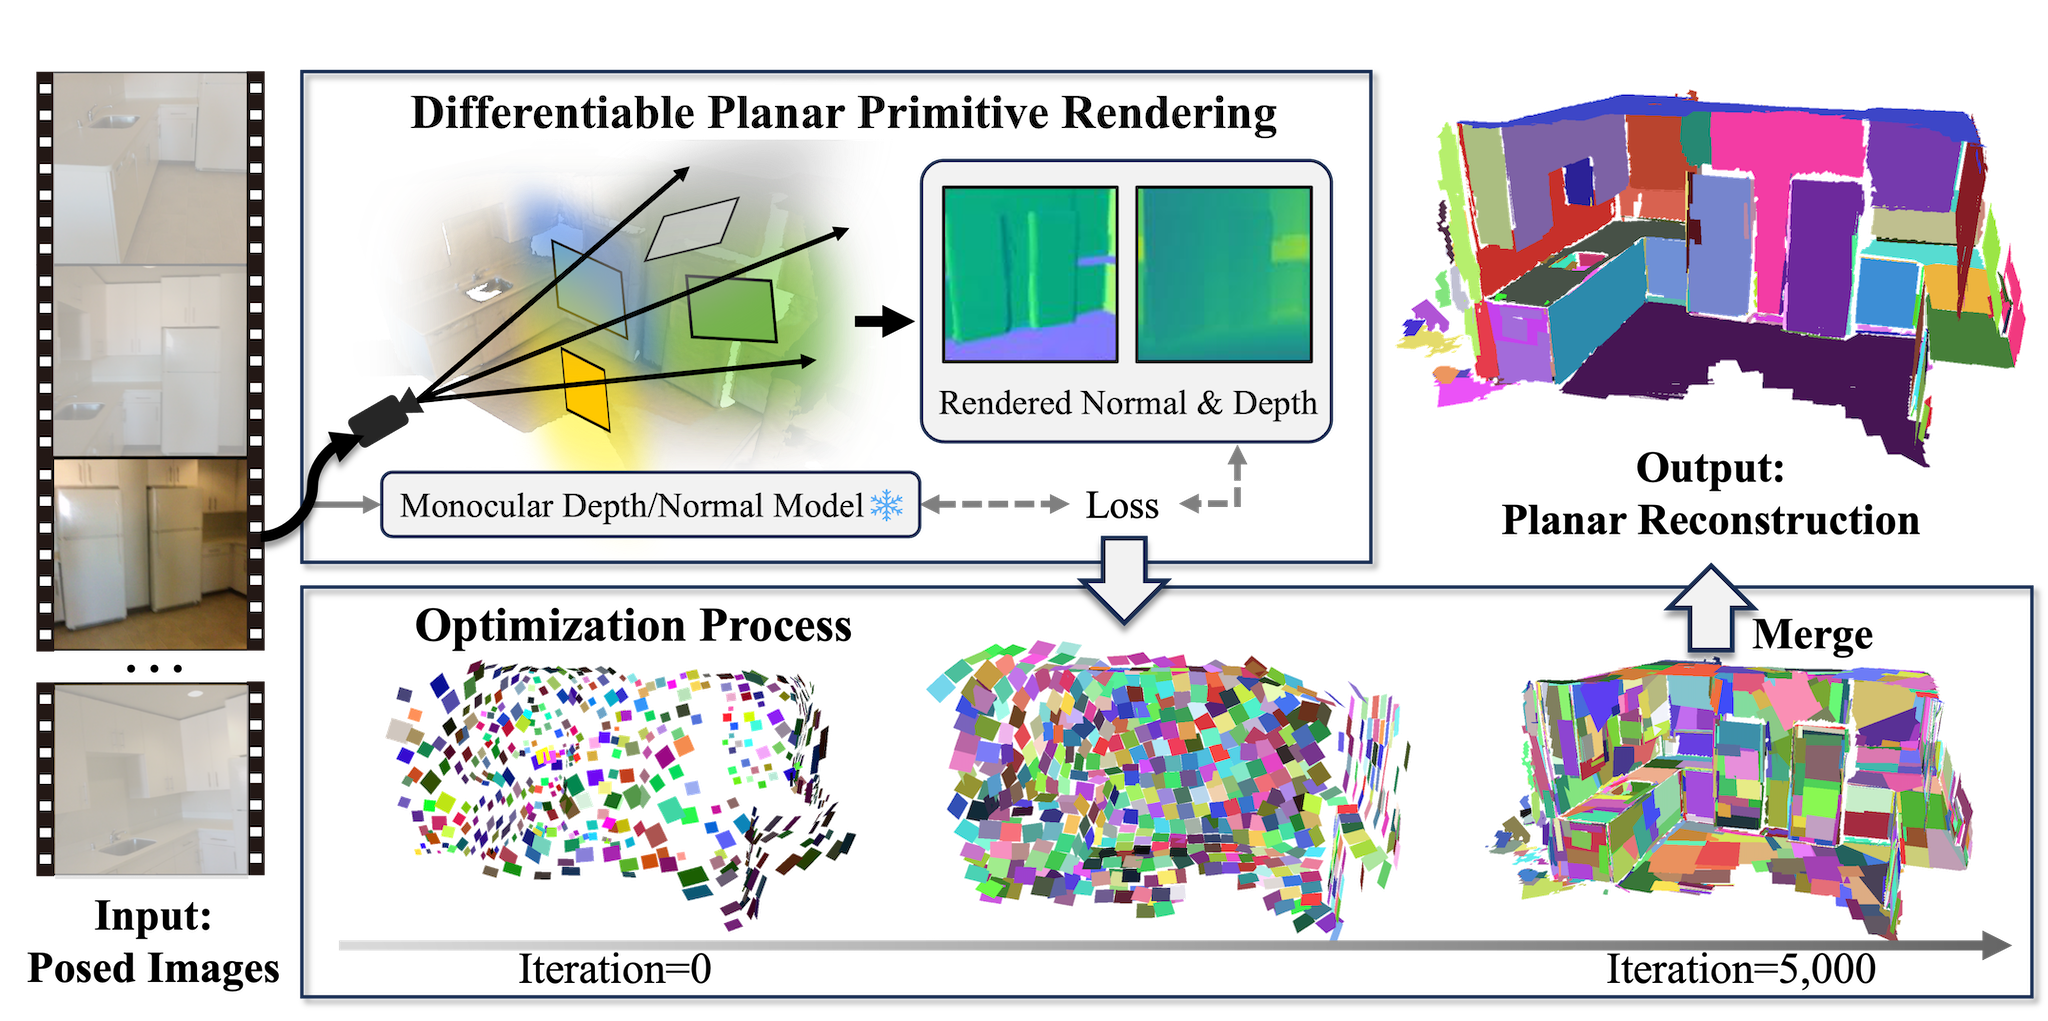
\includegraphics[width=0.95\textwidth]{images/planarsplatting.png}
    \caption{Arquitectura general de PlanarSplatting. El método optimiza primitivas planas 3D directamente desde imágenes multi-vista empleando renderizado diferenciable. Esto permite evadir la densificación clásica de MVS y obtener modelos ultrarrápidos (Fuente: \cite{tan2024planarsplatting}).}
    \label{fig:planarsplatting}
\end{figure}

En síntesis, la inyección de restricciones planas permite:
\begin{itemize}
    \item Reconstruir la superficie en tiempos ínfimos (minutos).
    \item Eliminar por completo la dependencia del MVS clásico para la inicialización.
    \item Extraer directamente mallas con texturas limpias y sin "geometría basura", ideales para la reconstrucción urbana masiva.
\end{itemize}

% ---------------------------------------------------------
% COMENTARIOS PARA EL USUARIO
% [NOTA PARA EL USUARIO: He reestructurado todo cronológicamente y temáticamente siguiendo tu estilo.
% El documento ahora fluye desde el problema (MVS y SfM lentos), hacia la solución parcial (NeRF/3DGS),
% luego el arreglo de la inicialización (DUSt3R) y terminamos con la abstracción geométrica y planar
% (PlaneRCNN -> GlueStick -> ZeroPlane -> PlanarSplatting) para cerrar el ciclo top-down.
% He dejado bullet points al final de los conceptos densos para fijar ideas de forma rápida, como me pediste.
%
% ¿He capturado bien el flujo resolutivo para el problema de reconstrucción urbana, si?
% Avísame si quieres que mantengamos algo de SLAM u otras referencias que quité para priorizar este hilo argumental.]
\chapter{Marco Teórico}

Este capítulo establece las bases teóricas de nuestra arquitectura \textit{top-down} para reconstrucción 3D a escala urbana. Vamos a ir paso a paso, desde cómo una cámara proyecta el mundo en 2D, pasando por cómo calculamos dónde está la cámara, hasta entender por qué los métodos clásicos como MVS se vuelven demasiado pesados. A partir de ese problema, introducimos las herramientas que nos permiten solucionarlo: alineación geométrica asíncrona, restricciones estructurales y el uso de modelos de inteligencia artificial para ir directo a la geometría útil (mallas ligeras) sin pasar por el costoso modelado píxel por píxel.

% TODO: Añadir aquí un bullet point o pequeño diagrama textual si es necesario para resumir la arquitectura general del capítulo y facilitar la lectura.

\section{Geometría Computacional y Formación de la Imagen}

\subsection{Modelo de Cámara Pinhole y Proyección Perspectiva}
El modelo de cámara \textit{pinhole} (o estenopeica) es el concepto fundamental que usamos para entender cómo un punto 3D del mundo real termina viéndose en una imagen 2D. Funciona a través de proyectar rayos de luz a través de un solo punto central hacia un plano de imagen. 

% TODO: Definir formalmente la matriz intrínseca (K) y extrínseca [R|t]. 
% TODO: Formular la proyección geométrica del punto 3D al plano bidimensional.

\subsection{Geometría Epipolar y Restricciones Multivista}
La geometría epipolar sirve para relacionar lo que ven dos cámaras mirando una misma escena. Si tenemos un punto en la primera imagen, la geometría epipolar nos dice que ese mismo punto en la segunda imagen debe estar en algún lugar a lo largo de una línea específica (línea epipolar). Esto es clave porque reduce nuestra búsqueda de correspondencias de 2D (buscar en toda la imagen) a 1D (buscar solo sobre esa línea).

% TODO: Explicar la Matriz Esencial (E) y Fundamental (F) conceptualmente. Asegurarse de mantener la formulación ligera y EVITAR LA MATEMÁTICA DENSA.
% TODO: Mencionar la restricción epipolar de forma directa y clara.

\section{Herramientas Matemáticas y Transformaciones}

\subsection{Descomposición en Valores Singulares (SVD)}
La Descomposición en Valores Singulares (SVD) es algo llamado factorización de matrices, que sirve para descomponer cualquier matriz compleja en partes más manejables. En visión computacional la usamos constantemente para resolver sistemas de ecuaciones lineales de forma robusta, como cuando queremos estimar matrices de rotación o calcular homografías.

Una desventaja de usar SVD es que, computacionalmente, es una operación pesada si las dimensiones de nuestras matrices crecen demasiado.

% TODO: Desarrollar la explicación de SVD, enfocándose en qué problema resuelve, cómo funciona y su aplicación específica en la optimización geométrica de este proyecto.

\subsection{Homografías (Transformaciones Proyectivas 2D-2D)}
Una homografía es una transformación que mapea puntos de un plano en una imagen a puntos de ese mismo plano visto desde otra imagen. Sirve para, por ejemplo, "pegar" o alinear dos fotos que ven una misma pared o el suelo desde distintos ángulos.

% TODO: Añadir la formulación algebraica básica (H) y detallar cómo se calcula a partir de correspondencias de puntos (vinculándolo al uso de SVD o DLT).

\section{Extracción de Información Visual}

\subsection{Deep Features vs SIFT Clásico}
Para saber que un píxel en una imagen es el mismo que en otra imagen, necesitamos extraer características o descriptores (\textit{features}). Clásicamente, algoritmos como SIFT funcionaban buscando esquinas o gradientes locales y les asignaban un descriptor matemático.

Actualmente, las \textit{Deep Features} (características extraídas mediante redes neuronales) logran este objetivo de forma mucho más robusta frente a cambios drásticos de iluminación o falta de textura. La diferencia es que, mientras SIFT entiende el píxel de forma aislada y local, las redes neuronales entienden un contexto semántico mucho más amplio. Una desventaja de las \textit{Deep Features} es que, para ser tan robustas, necesitan pasadas por redes neuronales pesadas, haciéndolas más lentas que los métodos clásicos si no se dispone de hardware dedicado.

% TODO: Expandir las ventajas y desventajas de ambos enfoques (robustez vs costo computacional) e incluir un resumen de viñetas al final de la sección.

\section{Estimación de Estado y Optimización Visual}

\subsection{Problema Perspective-n-Point (PnP) para Tracking}
El problema PnP busca responder a la pregunta pragmática: "si conozco las coordenadas 3D de ciertos puntos y sé dónde caen en mi imagen 2D, ¿dónde está mi cámara?". Resolver esto sirve para hacer \textit{tracking}, es decir, seguir la pose exacta de la cámara ($SE(3)$) frame a frame mientras la cámara se mueve por la ciudad.

% TODO: Explicar métodos de resolución algebraicos (DLT, P3P) y cómo los hacemos robustos (ej. RANSAC) cuando hay correspondencias falsas (outliers).

\subsection{Calibración y Bundle Adjustment}
Una vez que tenemos una estimación inicial de dónde están nuestros puntos 3D y nuestras cámaras, lo juntamos con un proceso de optimización no lineal llamado \textit{Bundle Adjustment}. Este algoritmo funciona ajustando conjuntamente todos los parámetros para minimizar el error entre dónde dijimos que caería el punto y dónde cayó realmente en la imagen (error de reproyección).

% TODO: Profundizar en las implicancias geométricas de trabajar con una cámara calibrada vs no calibrada, y detallar el proceso de optimización.

\section{El Paradigma Clásico de Reconstrucción (Bottom-Up)}

\subsection{Structure-from-Motion (SfM) y Triangulación}
SfM toma todo lo visto anteriormente y construye una nube de puntos rala. Funciona triangulando las observaciones a través de múltiples vistas para calcular la profundidad. El problema es que esta geometría inicial sirve para darnos una idea estructural de la escena, pero carece de la conectividad para formar mallas limpias.

% TODO: Detallar el flujo de generación inicial y por qué no es suficiente por sí solo para la reconstrucción final de mallas estructuradas.

\subsection{Multi-View Stereo (MVS) y sus Limitaciones}
Para rellenar los vacíos generados por SfM, el enfoque clásico aplica MVS. MVS intenta densificar la nube calculando la profundidad para todos los píxeles de la imagen mediante la comparación de múltiples vistas (fotoconsistencia).

Una desventaja grande de MVS es que, con el fin de ser exhaustivo, es computacionalmente intratable para escalas urbanas masivas. Genera redundancia de datos y mucha "geometría basura", como ruido en superficies reflectantes o árboles. Es por este motivo que escalar un modelo \textit{bottom-up} resulta ineficiente.

% TODO: Detallar brevemente el concepto de fotoconsistencia cuidando de ELIMINAR CUALQUIER MATEMÁTICA DENSA relacionada.

\section{Alineación de Trayectorias y Restricciones Geométricas}

\subsection{Transformaciones de Similitud Sim(3) y Recuperación Visual}
Cuando mapeamos una ciudad, procesamos múltiples grabaciones de video que nos generan trayectorias aisladas. Para juntar estos submapas sin sufrir por la acumulación de errores de escala (deriva), usamos transformaciones de similitud $Sim(3)$. Estas transformaciones funcionan ajustando la rotación, traslación y escala de golpe, lo que permite alinear los "espaguetis" de trayectorias en un mapa global asíncrono sin tener que re-optimizar toda la ciudad.

% TODO: Formular la corrección de deriva y explicar la ventaja de tener complejidad O(M) en la integración asíncrona.

\subsection{Restricciones Geométricas: Coplanaridad y Manhattan-world}
Para evitar que nuestra malla reconstruida dependa exclusivamente del escaneo visual ruidoso, imponemos reglas previas sobre cómo funciona la arquitectura real en las ciudades. Esto se conoce como la hipótesis \textit{Manhattan-world}. Asumimos que la gran mayoría de las estructuras urbanas están compuestas por superficies que son planas (coplanaridad) y que además, estas superficies suelen ser ortogonales o paralelas entre sí. Que juntos permiten filtrar el ruido y forzar modelos regulares y limpios.

% TODO: Explicar cómo integramos estas restricciones para obligar a la geometría final a ser ordenada.

\section{Abstracción Geométrica y Modelos Fundacionales (Enfoque Top-Down)}

\subsection{Modelos de Segmentación Semántica}
En lugar de reconstruir ciegamente geometría que no nos importa, utilizamos modelos fundacionales recientes (como Segment Anything Model - SAM). Esto sirve para priorizar regiones semánticas relevantes (como fachadas de edificios) e ignorar zonas problemáticas y dinámicas (como el cielo, los vehículos o los peatones), ahorrando poder de cómputo.

% TODO: Elaborar sobre el uso de priors semánticos y su integración en el pipeline de reconstrucción.

\subsection{Extracción Topológica: Planos y Esquemas Alámbricos}
Aquí es donde concretamos la visión \textit{top-down}. En lugar de crear nubes densas, usamos redes neuronales para analizar la imagen en 2D y detectar la estructura fundamental, como líneas largas, esquinas de edificios y esquemas alámbricos (wireframes). Toda esta información geométrica rala, una vez que la cruzamos con nuestras posiciones estimadas de la cámara en $SE(3)$, nos sirve para triangular directamente los nodos estructurales y sintetizar de forma algebraica una malla poligonal limpia, lista para ser texturizada.

% TODO: Explicar cómo la inferencia 2D se transforma directamente en una malla, y cerrar con un resumen de todo el proceso.
\chapter{Marco Metodológico: Arquitectura General del Sistema}

Los algoritmos actuales de reconstrucción, como Multi View Stereo (MVS), operan bajo un paradigma de densificación exhaustiva. El problema principal de este enfoque es que resulta excesivamente costoso y redundante computacionalmente, ya que intenta densificar millones de píxeles sin entender la estructura de lo que está reconstruyendo. Generar estas nubes masivas se vuelve inmanejable para entornos urbanos a gran escala.

Para solucionar esto, el sistema propuesto plantea un modelo basado firmemente en la abstracción semántica y geométrica. En lugar de procesar a ciegas la profundidad, el enfoque busca comprender primero la escena arquitectónica para luego triangular únicamente las primitivas estructurales necesarias. 

Este capítulo presenta un resumen rápido y estructurado de las fases que conforman la arquitectura propuesta, delineando la idea general del proyecto. Los detalles matemáticos y la implementación técnica profunda de cada fase se abordarán con muchísimo detalle en los capítulos posteriores.

\section{Pipeline de Reconstrucción}
El \textit{pipeline} propuesto abandona por completo la densificación clásica basada en píxeles. Esto funciona dividiendo el problema en fases secuenciales, priorizando en todo momento la extracción de caras y fronteras arquitectónicas.

\subsection{Fase 1: Preprocesamiento y Enmascaramiento Dinámico}
Esta fase sirve para limpiar las secuencias de video de información no deseada. Funciona a través de modelos de inferencia rápida, como FastSAM o YOLO, los cuales detectan objetos dinámicos dentro de la escena (típicamente autos y peatones), tal como se ejemplifica en la Figura \ref{fig:yolo_masking}.

\begin{figure}[H]
    \centering
    \begin{minipage}{0.48\textwidth}
        \centering
        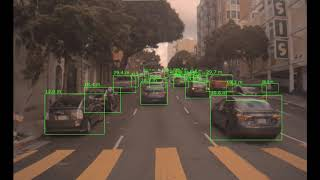
\includegraphics[width=\linewidth]{images/yolo_masking.png}
    \end{minipage}\hfill
    \begin{minipage}{0.48\textwidth}
        \centering
        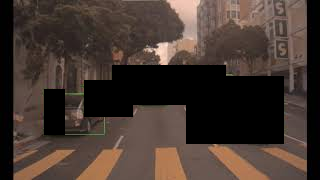
\includegraphics[width=\linewidth]{images/yolo_blacked.png}
    \end{minipage}
    \caption{Proceso de preprocesamiento: Identificación de elementos dinámicos con YOLO (izquierda) y su posterior enmascaramiento o censura espacial (derecha) para evitar ruido en la geometría (Fuente: Adaptado de \url{https://youtu.be/ftsUg5VlzIE}).}
    \label{fig:yolo_masking}
\end{figure}

Una vez identificados, se aplica un enmascaramiento dinámico (\textit{Masking}) para omitir estas regiones temporalmente de los cálculos geométricos. Un enfoque alternativo que muchos podrían sugerir es rellenar estos vacíos utilizando técnicas de \textit{Video Inpainting} previo a la reconstrucción. Sin embargo, como lo advierte la literatura en sistemas de mapeo dinámico \cite{bescos2018dynaslam}, la desventaja crítica del \textit{inpainting} generativo no es su tiempo de cómputo, sino su \textbf{inestabilidad geométrica}. 

Estos modelos \textit{alucinan} texturas visualmente plausibles pero carentes de consistencia temporal. Esta inestabilidad genera parpadeos y características falsas entre \textit{frames} que terminan corrompiendo de forma irremediable la geometría epipolar y el rastreo (\textit{tracking}) de la cámara.

\begin{itemize}
    \item \textbf{Resumen:} Se usan modelos de segmentación rápida para enmascarar y descartar los objetos móviles, optando por ignorar la información en lugar de inventarla con \textit{inpainting}, salvaguardando así la pureza matemática del sistema.
\end{itemize}

\subsection{Fase 2: Extracción Estructural y Tracking Híbrido}
El objetivo de esta fase es rastrear la trayectoria de la cámara y obtener la estructura base evadiendo los descriptores clásicos basados en texturas, como SIFT o ORB, porque son propensos a fallar en entornos repetitivos o sin textura. 

Se utilizan arquitecturas neuronales de última generación, como Co-PLNet \cite{wang2026coplnet}, para extraer nodos clave y los \textit{wireframes} estructurales en cada imagen. Como se observa en la Figura \ref{fig:coplnet_examples}, la red identifica con precisión las esquinas y líneas arquitectónicas de la edificación. 

\begin{figure}[H]
    \centering
    \begin{minipage}{0.48\textwidth}
        \centering
        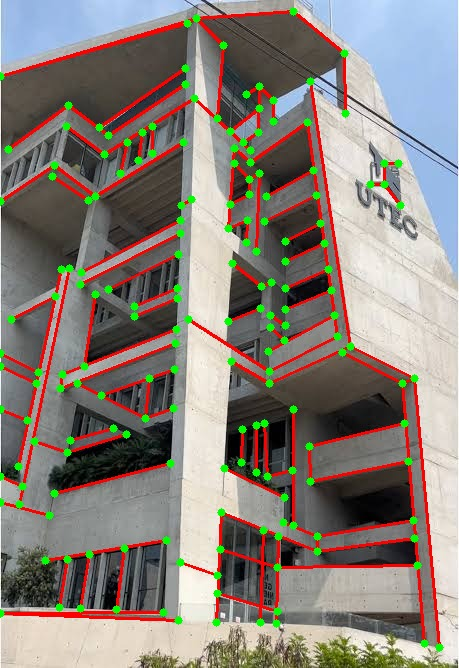
\includegraphics[width=\linewidth]{images/coplnet_utec1.png}
    \end{minipage}\hfill
    \begin{minipage}{0.48\textwidth}
        \centering
        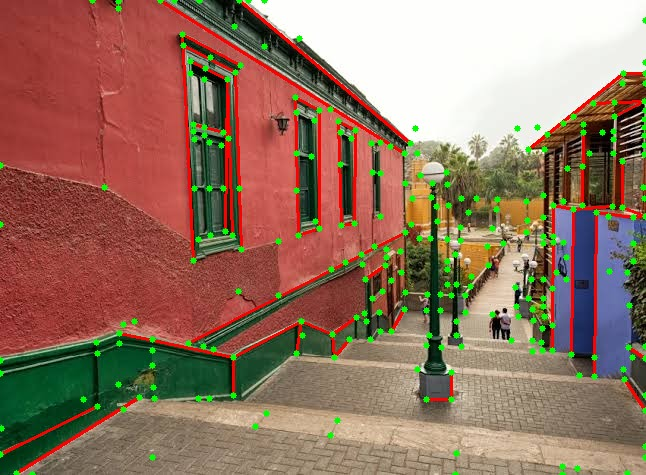
\includegraphics[width=\linewidth]{images/coplnet_barranco.png}
    \end{minipage}
    \caption{Demostración de extracción conjunta de puntos y líneas sobre edificaciones reales utilizando Co-PLNet. Se observan los nodos estructurales en verde y las fronteras arquitectónicas en rojo (Fuente: Elaboración propia).}
    \label{fig:coplnet_examples}
\end{figure}

Posteriormente, se aplican arquitecturas de grafos, específicamente GlueStick \cite{pelaez2023gluestick}, para realizar un emparejamiento robusto conjunto de puntos y líneas. Esto permite calcular una triangulación dispersa inicial que estima la pose de la cámara.

\subsection{Fase 3: Segmentación y Detección de Caras (Planos)}
En esta etapa, el sistema inyecta restricciones semánticas para detectar y segmentar los planos arquitectónicos dominantes usando modelos especializados como ZeroPlane \cite{liu2025zeroplane}, PlaneRCNN \cite{liu2019planercnn}, o combinaciones robustas usando DUSt3R \cite{wang2024dust3r} y SAM. Como se ejemplifica en la Figura \ref{fig:plane_segmentation}, estas arquitecturas son capaces de identificar y aislar matemáticamente las distintas instancias planas que componen la escena.

\begin{figure}[H]
    \centering
    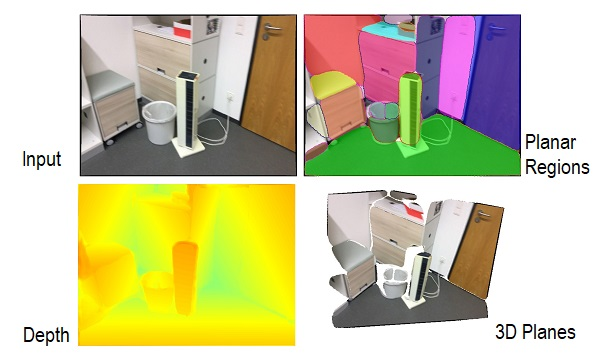
\includegraphics[width=0.95\textwidth]{images/planercnn_segmentation.jpg}
    \caption{Demostración de segmentación de superficies planares. La imagen ilustra cómo la red infiere máscaras para cada instancia plana detectada. Cada color representa un plano geométrico distinto, facilitando la distinción entre superficies arquitectónicas y elementos ajenos (Fuente: \cite{liu2019planercnn}).}
    \label{fig:plane_segmentation}
\end{figure}

Analíticamente, la segmentación de planos proporciona restricciones geométricas severas para la reconstrucción. Como se aprecia en la Figura \ref{fig:plane_segmentation}, al asignar a cada píxel su pertenencia a una instancia plana específica, el sistema discrimina las superficies puramente arquitectónicas (fachadas, calzadas, muros) de las geometrías de alta entropía (como vegetación o mobiliario urbano). Esta clasificación semántica permite que las geometrías complejas sean excluidas de la optimización del plano infinito, encapsulándolas temporalmente en volúmenes delimitadores (\textit{bounding boxes}) para evitar que su topología irregular corrompa la instanciación matemática de las caras principales.

\begin{itemize}
    \item \textbf{Resumen:} Se aíslan las caras planares útiles de las geometrías complejas garantizando que solo la estructura puramente arquitectónica guíe la reconstrucción 3D.
\end{itemize}

\subsection{Fase 4: Completado de Caras y Fusión Temporal}
El reto en este punto es lograr mallas continuas a partir del flujo de video. Esto se soluciona fusionando temporalmente las caras segmentadas que apuntan al mismo plano físico a lo largo de los \textit{frames}.

Sobre estos \textit{super-segmentos} fusionados, el sistema recupera los puntos estructurales conocidos provenientes del \textit{wireframe} (Fase 2). La hipótesis técnica radica en que, al reconocer estas caras semánticas, podemos utilizar los nodos estructurales que habitan en ellas para completarlas matemáticamente. Con esos vértices estructurales proyectados, se aplica el algoritmo robusto LO-RANSAC \cite{lebeda2012loransac} para extraer la ecuación final del muro.

% TODO: [Aquí se detallarán las matemáticas de LO-RANSAC en su respectivo capítulo de implementación]

\subsection{Fase 5: Extracción de Fronteras y Texturizado}
RANSAC devuelve una abstracción matemática infinita. Esta fase sirve para delimitar físicamente esa superficie utilizando las líneas proyectadas del \textit{wireframe} (Fase 2) para recortar el plano infinito, estableciendo las fronteras reales del muro.

Una vez instanciado este polígono 3D cerrado y finito, se le aplica el texturizado. Para garantizar un mapeo UV de alta fidelidad, se hace uso de una homografía directa desde el fotograma que se encuentre más ortogonal a la normal del plano.

% TODO: [Aquí se detallará la ecuación de la homografía H en el capítulo correspondiente]

\begin{itemize}
    \item \textbf{Resumen:} Las líneas del wireframe recortan el plano infinito creando el modelo 3D final, que luego es pintado con el fotograma más alineado posible de esa pared.
\end{itemize}

\section{Infraestructura de la Base de Datos de Poses y Alineación Topológica}
La captura asíncrona de datos urbanos a gran escala genera múltiples secuencias de video independientes, las cuales resultan en sub-mapas locales o trayectorias de cámara inconexas. Para unificar esta información y dotar al sistema de persistencia espacial, se establece una infraestructura de base de datos de poses centralizada (\textit{Pose Database}).

El desafío fundamental radica en la alineación topológica de estas trayectorias locales hacia un sistema de coordenadas global coherente. A nivel algorítmico, esto requiere la resolución de un problema de Optimización de Grafo de Poses (\textit{Pose Graph Optimization}, PGO). Cuando existen co-visibilidades entre diferentes secuencias de video (es decir, cierres de bucle entre sub-mapas), el sistema extrae coincidencias y computa transformaciones de similitud $Sim(3)$ ---las cuales ajustan la rotación, traslación y escala de forma simultánea--- para anclar matemáticamente las trayectorias relativas.

Para mitigar la acumulación de error inercial y de escala (\textit{drift}), intrínseco al rastreo monocular en distancias prolongadas, la infraestructura integra datos de telemetría GPS que actúan como restricciones absolutas (\textit{absolute priors}) dentro del grafo de optimización. Esta arquitectura descentralizada y robusta garantiza la consistencia global a nivel metropolitano, facultando al sistema a asimilar y ensamblar continuamente nuevos fragmentos de la ciudad sin la penalidad computacional de tener que re-optimizar el mapa global desde cero.

%% ============================================================================
\nocite{*}
\printbibliography[title={\hfill\Large\bf{REFERENCIAS BIBLIOGRÁFICAS}\hfill}] 

%% ============================================================================
\appendix

\end{document}